\documentclass[1610,20pt]{beamer}
\usepackage{fontspec}
\usepackage{amsfonts}
\usepackage{tangocolors}
\usepackage{listings}
\usepackage{hyperref}
\usepackage{multicol}
\usepackage{enumitem}

\usepackage{tikz}
\usetikzlibrary{shapes}

% thanks http://en.wikibooks.org/wiki/LaTeX/Packages/Listings
\newcommand\normallistingstyle{\lstset{ %
  %language=Python,                % the language of the code
  basicstyle=\footnotesize\ttfamily,
                                   % the size of the fonts that are used for the code
  %numbers=left,                   % where to put the line-numbers
  %numberstyle=\tiny\color{gray},  % the style that is used for the line-numbers
  %stepnumber=1,                   % the step between two line-numbers. If it's 1, each line 
                                  % will be numbered
  %numbersep=5pt,                  % how far the line-numbers are from the code
  backgroundcolor=\color{white},      % choose the background color. You must add \usepackage{color}
  showspaces=false,               % show spaces adding particular underscores
  showstringspaces=false,         % underline spaces within strings
  showtabs=false,                 % show tabs within strings adding particular underscores
  %frame=single,                   % adds a frame around the code
  rulecolor=\color{black},        % if not set, the frame-color may be changed on line-breaks within not-black text
  tabsize=2,                      % sets default tabsize to 2 spaces
  %captionpos=b,                   % sets the caption-position to bottom
  breaklines=true,                % sets automatic line breaking
  breakatwhitespace=false,        % sets if automatic breaks should only happen at whitespace
  title=\ ,
  emph={[2]__import__,range,input,raw_input,NameError,dir,dict},
  keywordstyle=\color{ta3chocolate},          % keyword style
  commentstyle=\color{ta3orange},       % comment style
  stringstyle=\color{ta3orange},         % string literal style
  emphstyle={[2]\color{ta2orange}},
  %escapeinside=\$\$,            % if you want to add LaTeX within your code
  morekeywords={*,...}               % if you want to add more keywords to the set
  aboveskip=0pt,
  belowskip=0pt,
}}
\newcommand\biglistingstyle{\lstset{ %
    basicstyle=\small,
}}
\newcommand\altlistingstyle{\lstset{ %
    backgroundcolor=\color{black},
    basicstyle=\small\color{white},
    keywordstyle=\color{tachocolate},
    commentstyle=\color{tachameleon},
    stringstyle=\color{tachameleon},
    emphstyle={[2]\color{tabutter}},
    emphstyle={[3]\color{taorange}},
}}
\normallistingstyle
\newcommand\topshade{
    \begin{tikzpicture}[remember picture,overlay]
    \fill[black] (current page.west) rectangle +(100cm, -100cm);
    \end{tikzpicture}
    \vspace{-50pt}
    \biglistingstyle
}
\newcommand\halfshadenopause{
    \altlistingstyle\bigskip\bigskip\bigskip
}
\newcommand\halfshade{
    \pause\halfshadenopause
}
\newcommand\bottomshade{
    \normallistingstyle
}

\definecolor{fedblue}{rgb}{0.23529411764705882, 0.43137254901960786, 0.6666666666666666}
\definecolor{fedgray}{rgb}{0.8705882352941177, 0.8705882352941177, 0.8705882352941177}
\definecolor{mutegray}{rgb}{0.7705882352941177, 0.7705882352941177, 0.7705882352941177}

\newcommand\sk{\par\bigskip\bigskip\par}
\newcommand\wh[1]{\only<#1>{\color{white}}}
\newcommand\tx[2]{\alt<#1>{\textcolor{ta3gray}}{\textcolor{ta3gray}}{\uncover<#1->{#2}}}
\newcommand\rd[2]{\alt<#1>{\textcolor{taskyblue}}{\textcolor{ta3gray}}{#2}}
\renewcommand\emph[1]{\textcolor{fedblue}{#1}}

%\setbeamertemplate{footline}[text line]{%
%  \parbox{\linewidth}{\vspace*{-8pt}\textcolor{fedgray}{Petr Viktorin - @encukou\hfill}}}
%\setbeamertemplate{navigation symbols}{}

\begin{document}
\fontspec[Numbers=Lining]{Fertigo Pro}
\color{ta3gray}

\begin{center}
\title{Pyvo přednáška}
\author{Petr Viktorin}
\date{\today}
% 
% {\setbeamercolor{background canvas}{bg=tascarletred}
% \frame{\color{white}
%     \textcolor{white}{Python Language Summit only}
%     \sk
%     \textcolor{white}{Please don't redistribute this version of the slides}
% }
% }

\begin{frame}[fragile]
    Color check

    {\color{mutegray} Is this readable? }
\end{frame}

{\setbeamercolor{background canvas}{bg=fedblue}
\frame{\color{fedgray}
    \sk
    \textcolor{fedgray}{Python Packaging in Fedora}
    \sk\sk
    \textcolor{fedgray}{Petr Viktorin}\\[-0.25cm]
    \textcolor{fedgray}{\tiny pviktori@redhat.com}
    \sk
    \textcolor{fedgray}{\tiny Flock, 2016-08-02}
}
}

\begin{frame}[fragile]
    
\includegraphics[width=0.9\textwidth]{fedora-loves-python}
\end{frame}

{\setbeamercolor{background canvas}{bg=fedblue}
\begin{frame}[fragile]
    \huge\color{white}
    I. Python 3
\end{frame}
}

\begin{frame}[fragile]
    \small
    \begin{tabular}{rl}
    Python & 1991 \\
    \color{mutegray} Java & \color{mutegray} 1995 \\
    \pause~\\
    Python 3.0 & 2008 \\
    \color{mutegray} Node.js & \color{mutegray} 2009 \\
    \pause~\\
    Python 3.5 & 2015 \\% -09-13 \\
    %\pause
    %\color{mutegray} Fedora 23 Alpha Freeze & \color{mutegray} 2015-08-11 \\
    \pause~\\
    Python 2 EOL & 2020 \\
    \end{tabular}
\end{frame}

\begin{frame}[fragile]
    Python 3 Porting Database

    \sk\sk

    http://fedora.portingdb.xyz
\end{frame}

\begin{frame}[fragile]
    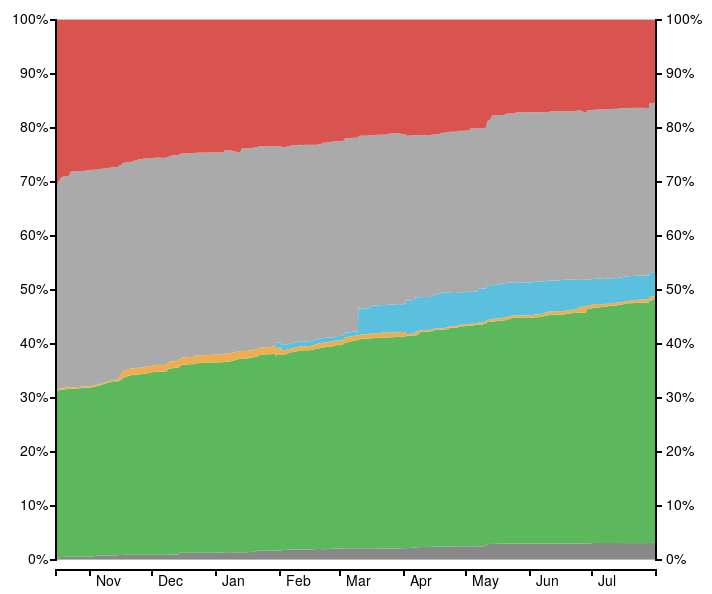
\includegraphics[width=0.8\textwidth]{history-graph}

    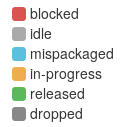
\includegraphics[width=0.2\textwidth]{history-legend}

    %\tiny Details: fedora.portingdb.xyz
\end{frame}

\begin{frame}[fragile]
    ~{\color{mutegray}at least}~ \\
    {\huge ~49,9\%}     % 1446 / 3178

    of Python software \\
    packaged in Fedora \\
    supports Python 3
    \sk\pause
    {\huge ~45,5\%} % (1446 + 139) / 3178 

    has the Py 3 version \emph{\textit{packaged}}
\end{frame}

\begin{frame}[fragile]
    Help us port!

    
\includegraphics[width=0.6\textwidth]{parselmouth3}

    http://fedora.portingdb.xyz
\end{frame}

\begin{frame}[fragile]
    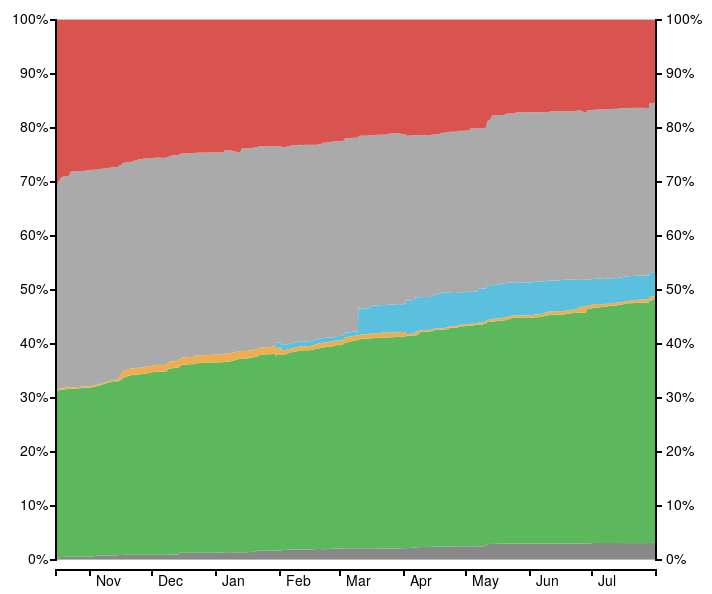
\includegraphics[width=0.9\textwidth]{history-graph}
\end{frame}

\begin{frame}[fragile]
    
\includegraphics[width=0.1\textwidth]{koji-icon} ~~~
    
\includegraphics[width=0.1\textwidth]{bodhi-logo}\\
    Fedora infra

    \sk

%     
\includegraphics[width=0.1\textwidth]{mercurial} ~~~
%     
\includegraphics[width=0.1\textwidth]{bazaar-logo} ~~~
%     
\includegraphics[width=0.1\textwidth]{trac_bullet} \\
%     Version Control

    
\includegraphics[width=0.1\textwidth]{gtk} ~~~
    
\includegraphics[width=0.1\textwidth]{wx-logo} ~~~
    
\includegraphics[width=0.1\textwidth]{sugar} \\
    Desktop toolkits

    \sk

    
\includegraphics[width=0.12\textwidth]{gimp} ~~~
    
\includegraphics[width=0.1\textwidth]{inkscape-logo} ~~~
    
\includegraphics[width=0.4\textwidth]{Logo_Samba} \\
    Big non-Python apps

\end{frame}

{\setbeamercolor{background canvas}{bg=fedblue}
\begin{frame}[fragile]~
    {\color{mutegray} I. Python 3}

    \sk\color{white}

    \huge
    II. Automating Packaging
\end{frame}
}

\begin{frame}[fragile]
    A packager should:
    \small

    \begin{itemize}
    \item{1.} Make sure SW plays nice
    \item{2.} Integrate with rest of system
    \item{3.} Check licenses, patents, etc.
    \pause
    \item{4.} Read 50 pages of guidelines
    \item{5.} Know a weird macro language
    \end{itemize}
\end{frame}

\begin{frame}[fragile]
    \begin{lstlisting}[frame=single]
%global pypi_name mypkg

Name:           python-%{pypi_name}
Version:        2.4.25.1
Release:        1%{?dist}

License:        Python
URL:            https://github.com/%{pypi_name}/%{pypi_name}
Source0:        https://pypi.python.org/packages/source/p/%{pypi_name}/%{pypi_name}-%{version}.tar.gz
    \end{lstlisting}
    \sk\sk
\end{frame}
 
\begin{frame}[fragile]
    \begin{lstlisting}[frame=single]
%if 0%{?rhel} && 0%{?rhel} <= 6
%{!?__python2:        %global \ __python2 /usr/bin/python2}
%{!?python2_sitelib:  %global \ python2_sitelib %(%{__python2} -c 
%endif

%if 0%{?fedora} > 12 || 0%{?rhel} >
%global with_python3 1

%global __python3 python3
%endif
    \end{lstlisting}
    \sk\sk
\end{frame}

\begin{frame}[fragile]
    \begin{lstlisting}[frame=single]
from distutils.core import setup

setup(
  name='mypkg',
  version='2.4.25.1',
  author='Me',
  url='github.com/me/mypkg/',
  packages=['mypkg'],
  install_requires=['six'],
)
    \end{lstlisting}
    \sk\sk
\end{frame}

\begin{frame}[fragile]
    Enter pyp2rpm

    \begin{lstlisting}[frame=single]
# dnf install /usr/bin/pyp2rpm
$ pyp2rpm mypkg
    \end{lstlisting}

    \sk\pause
    \color{mutegray}
    It might actually work!
\end{frame}

\begin{frame}[fragile]
    ~{\color{mutegray} We can use pyp2rpm to...}

    \sk

    Auto-build all of PyPI in COPR!

    \sk\pause
    {\color{mutegray} Why?}
    \begin{itemize}
    \pause
    \item{-} Test pyp2rpm
    \pause
    \item{-} Run upstream tests
    \pause
    \item{-} Provide a repository
    \end{itemize}
\end{frame}

\begin{frame}[fragile]
    \begin{lstlisting}[frame=single]
dnf pip install -r requirements.txt
    \end{lstlisting}

    \sk

    \color{mutegray}(hypothetical command)
\end{frame}

\begin{frame}[fragile]
    \small
    \begin{tabular}{ccc}
    “PyPI” name & Fedora pkg \\
    \texttt{pyopencl} & \texttt{python3-pyopencl} \\
    \texttt{mypy-lang} & \texttt{python3-mypy} \\
    \end{tabular}

    \sk\pause

    \begin{lstlisting}[frame=single]
$ dnf repoquery --provides
                python3-pyopencl
...
python3.5dist(pyopencl) = 2015.2
...
    \end{lstlisting}

    \pause
    Live in Fedora 25!
\end{frame}

{\setbeamercolor{background canvas}{bg=fedblue}
\begin{frame}[fragile]~
    {\color{mutegray} I. Python 3} \\
    {\color{mutegray} II. Automating Packaging} \\

    \sk\color{white}

    \huge
    III. System Python
\end{frame}
}

\begin{frame}[fragile]
    System Python

    \sk

    \texttt{/usr/libexec/system-python}

    \sk

    An effort to minimize minimal installs \\
    (cloud images)
\end{frame}

\begin{frame}[fragile]
    Python stdlib by disk size
    \sk

    \includegraphics[width=0.9\textwidth]{stdlib-size}
\end{frame}

\begin{frame}[fragile]
    System Python libs
    \sk

    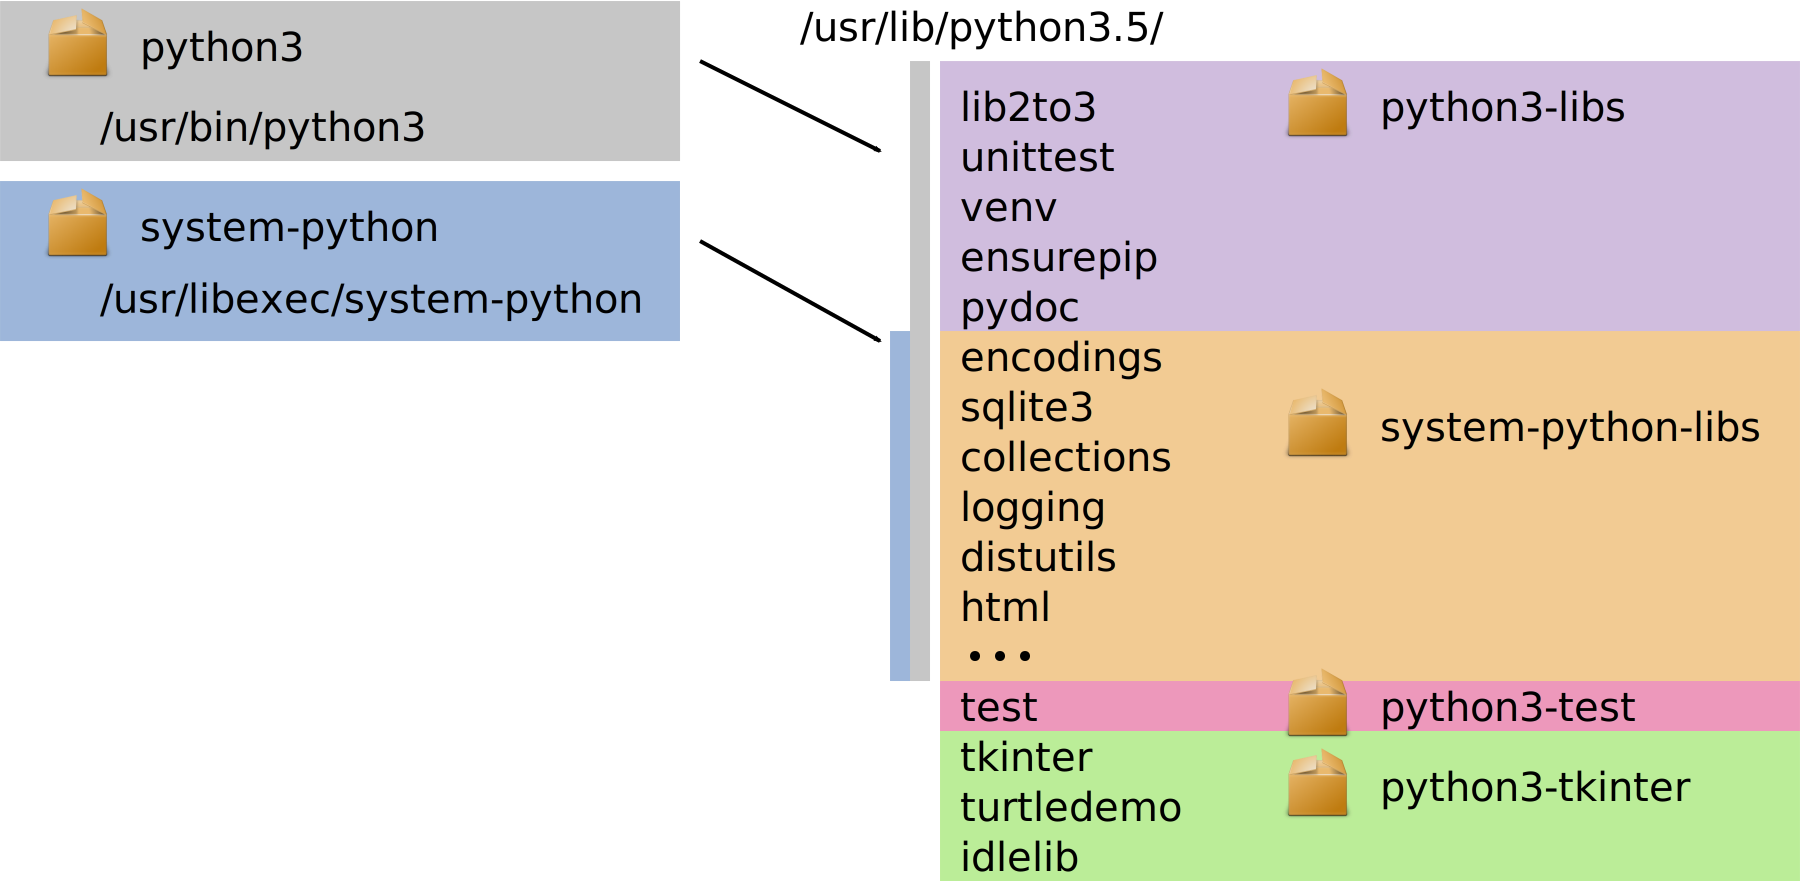
\includegraphics[width=0.9\textwidth]{system-python}
\end{frame}

\begin{frame}[fragile]
    Possible users: DNF, cloud-init

    \sk\pause

    Future: Isolation of system tools?
\end{frame}

{\setbeamercolor{background canvas}{bg=fedblue}
\begin{frame}[fragile]~
    {\color{mutegray} I. Python 3} \\
    {\color{mutegray} II. Automating Packaging} \\
    {\color{mutegray} III. System Python} \\

    \sk\color{white}

    \huge
    IV. Python 3.6
\end{frame}
}

\begin{frame}[fragile]
    Python 3.6

    \sk
    
    \small
    \begin{itemize}
    \item{*} Format Strings
    \item{*} Large Speedups
    \item{*} Advanced class creation tools
    \end{itemize}
\end{frame}

\begin{frame}[fragile]

    \small
    \begin{tabular}{rl}
    Python 3.6 Alpha 1 & 2016-05-17 \\
    \color{fedblue} Fedora 25 Alpha Freeze & \color{fedblue} 2016-08-09 \\
    \pause~\\
    Python 3.6 Beta 1 & 2016-09-12 \\
    \color{fedblue} Fedora 25 Beta Freeze & \color{fedblue} 2016-09-20 \\
    \pause~\\
    Python 3.6 RC 1 & 2016-12-05 \\
    \color{fedblue} Fedora 25 Final Freeze & \color{fedblue} 2016-10-25 \\
    \pause~\\
    Python 3.6 Final & 2016-12-05 \\
    \color{fedblue} Fedora 26 Branches& \color{fedblue} 2016-12-??? \\
    \end{tabular}
\end{frame}

{\setbeamercolor{background canvas}{bg=fedblue}
\begin{frame}[fragile]~
    {\color{mutegray} I. Python 3} \\
    {\color{mutegray} II. Automating Packaging} \\
    {\color{mutegray} III. System Python} \\
    {\color{mutegray} IV. Python 3.6} \\

    \sk\color{white}

    \huge
    V. Who's “we”?
\end{frame}
}

\begin{frame}[fragile]
    python-maint @ Red Hat
    \sk

    
\includegraphics[width=0.12\textwidth]{Join_OSDeveloper} ~~
    
\includegraphics[width=0.12\textwidth]{Join_OSDeveloper} ~~
    
\includegraphics[width=0.12\textwidth]{Join_OSDeveloper} ~~ 
    
\includegraphics[width=0.12\textwidth]{Join_OSDeveloper-no} ~~
    
\includegraphics[width=0.12\textwidth]{Join_OSDeveloper-no} ~~
    
\includegraphics[width=0.12\textwidth]{Join_OSDeveloper-no} ~~
    
\includegraphics[width=0.12\textwidth]{Join_OSDeveloper-no}
\end{frame}

\begin{frame}[fragile]
    python-maint @ Red Hat
    \sk

    
\includegraphics[width=0.12\textwidth]{Join_OSDeveloper} ~~
    
\includegraphics[width=0.12\textwidth]{Join_OSDeveloper} ~~
    
\includegraphics[width=0.12\textwidth]{Join_OSDeveloper} ~~ 
    
\includegraphics[width=0.12\textwidth]{Join_OSDeveloper-me} ~~
    
\includegraphics[width=0.12\textwidth]{Join_OSDeveloper-no} ~~
    
\includegraphics[width=0.12\textwidth]{Join_OSDeveloper-no} ~~
    
\includegraphics[width=0.12\textwidth]{Join_OSDeveloper-no}
\end{frame}

\begin{frame}[fragile]
    python-maint @ Red Hat
    \sk

    
\includegraphics[width=0.12\textwidth]{Join_OSDeveloper-x} ~~
    
\includegraphics[width=0.12\textwidth]{Join_OSDeveloper} ~~
    
\includegraphics[width=0.12\textwidth]{Join_OSDeveloper} ~~ 
    
\includegraphics[width=0.12\textwidth]{Join_OSDeveloper-me} ~~
    
\includegraphics[width=0.12\textwidth]{Join_OSDeveloper-no} ~~
    
\includegraphics[width=0.12\textwidth]{Join_OSDeveloper-no} ~~
    
\includegraphics[width=0.12\textwidth]{Join_OSDeveloper-no}
\end{frame}

\begin{frame}[fragile]
    python-maint @ Red Hat
    \sk

    
\includegraphics[width=0.12\textwidth]{Join_OSDeveloper-x} ~~
    
\includegraphics[width=0.12\textwidth]{Join_OSDeveloper} ~~
    
\includegraphics[width=0.12\textwidth]{Join_OSDeveloper} ~~ 
    
\includegraphics[width=0.12\textwidth]{Join_OSDeveloper-me} ~~
    
\includegraphics[width=0.12\textwidth]{Join_OSDeveloper} ~~
    
\includegraphics[width=0.12\textwidth]{Join_OSDeveloper-no} ~~
    
\includegraphics[width=0.12\textwidth]{Join_OSDeveloper-no}
\end{frame}

\begin{frame}[fragile]
    python-maint @ Red Hat
    \sk

    
\includegraphics[width=0.12\textwidth]{Join_OSDeveloper-x} ~~
    
\includegraphics[width=0.12\textwidth]{Join_OSDeveloper-x} ~~
    
\includegraphics[width=0.12\textwidth]{Join_OSDeveloper-x} ~~ 
    
\includegraphics[width=0.12\textwidth]{Join_OSDeveloper-me} ~~
    \includegraphics[width=0.12\textwidth]{Join_OSDeveloper} ~~
    \includegraphics[width=0.12\textwidth]{Join_OSDeveloper-no} ~~
    \includegraphics[width=0.12\textwidth]{Join_OSDeveloper-no}
\end{frame}

\begin{frame}[fragile]
    python-maint @ Red Hat
    \sk

    \includegraphics[width=0.12\textwidth]{Join_OSDeveloper-x} ~~
    \includegraphics[width=0.12\textwidth]{Join_OSDeveloper-x} ~~
    \includegraphics[width=0.12\textwidth]{Join_OSDeveloper-x} ~~ 
    \includegraphics[width=0.12\textwidth]{Join_OSDeveloper-me} ~~
    \includegraphics[width=0.12\textwidth]{Join_OSDeveloper} ~~
    \includegraphics[width=0.12\textwidth]{Join_OSDeveloper} ~~
    \includegraphics[width=0.12\textwidth]{Join_OSDeveloper}
\end{frame}

\begin{frame}[fragile]
    Sorry!

    \sk

    We'll do better!
\end{frame}

\begin{frame}[fragile]~
    {\large We're Python SIG}

    \sk

    python-devel\\{\small @lists.fedoraproject.org}

    \sk

    \#fedora-python on Freenode

    \sk

    fedora-python on Github
\end{frame}

{\setbeamercolor{background canvas}{bg=fedblue}
\begin{frame}[fragile]~
    {\color{mutegray} I. Python 3} \\
    {\color{mutegray} II. Automating Packaging} \\
    {\color{mutegray} III. System Python} \\
    {\color{mutegray} IV. Python 3.6} \\
    {\color{mutegray} V. Who's “we”?} \\
\end{frame}
}

\end{center}
\end{document}

